\documentclass[a4paper,11pt]{article}

\usepackage[T1]{fontenc}
\usepackage[utf8]{inputenc}
\usepackage{graphicx}
\usepackage{amsmath,amssymb,amsthm,textcomp}
\usepackage{enumerate}
\usepackage{multicol}
\usepackage{tikz}
\usepackage{geometry}
\usepackage{float}
\usepackage{hyperref}
\usepackage{url}
\usepackage[export]{adjustbox}
\usepackage[parfill]{parskip}
\usepackage{array}
\usepackage{titlesec}
\usepackage{fmtcount} % for \ordinalnum
\usepackage{array,multirow}
\usepackage[document]{ragged2e}
\usepackage{longtable}
\usepackage{hyperref}

%\usepackage{enumitem}
\PassOptionsToPackage{hyphens}{url}
\geometry{total={210mm,297mm},
left=25mm,right=25mm,top=20mm,bottom=20mm}

\linespread{1.2}

% custom footers and headers
\usepackage{fancyhdr}
\pagestyle{fancy}
\lhead{}
\chead{}
\rhead{}
\lfoot{FIT5147 Assignment 3 | Data Exploration}
\cfoot{}
\rfoot{Page \thepage}
\renewcommand{\headrulewidth}{0pt}
\renewcommand{\footrulewidth}{0pt}
%

% code listing settings
\usepackage{listings}
\lstset{
    language=Scala,
    basicstyle=\ttfamily\small,
    aboveskip={1.0\baselineskip},
    belowskip={1.0\baselineskip},
    columns=fixed,
    extendedchars=true,
    breaklines=true,
    tabsize=4,
    prebreak=\raisebox{0ex}[0ex][0ex]{\ensuremath{\hookleftarrow}},
    frame=lines,
    showtabs=false,
    showspaces=false,
    showstringspaces=false,
    keywordstyle=\color[rgb]{0.627,0.126,0.941},
    commentstyle=\color[rgb]{0.133,0.545,0.133},
    stringstyle=\color[rgb]{01,0,0},
    numbers=left,
    numberstyle=\small,
    stepnumber=1,
    numbersep=10pt,
    captionpos=t,
    escapeinside={\%*}{*)}
}

%\renewcommand{\thesubsubsection}{\thesubsection.\alph{subsubsection}}

\setcounter{secnumdepth}{3}
\begin{document}
%%%%% Title
\author{Student Name: \textbf{Vinh Phan} \\ Student Number: \textbf{27612937} \\\\}
\title{FIT5147 Data Exploration and Visualization \\ Assignment 3 \\ Data Exploration Report}
\date{\today}
\maketitle
\tableofcontents

%%%%% Begin of Document %%%%%
\section{Terminologies}
	\begin{tabular}{|>{\centering\arraybackslash}p{3cm}||>{\arraybackslash}p{11cm}|}
	\hline 
	\textbf{Terms} & \textbf{Description} \\ 
	\hline 
	Review & A review / feedback customers put in the feedback section of a product \\ 
	\hline 
	ASIN & Amazon product identification system \\ 
	\hline 
	Sales Rank & Amazon created a sales rank figure to rate a product \\ 
	\hline 
	Helpfulness & In a review, we can “like / dislike” it. By using the feature, we can see how valuable the review is \\ 
	\hline 
	Rating & The figure that customers rate for a particular product from the reviews \\ 
	\hline 
	Bag words & The list of unique words in a paragraph. In the document context, we combine all review texts, then remove less informative words / symbols, then save it to a bag words \\ 
	\hline 
	Single words & The word appears only one throughout the paragraph \\ 
	\hline 
	Frequent pattern & A data mining problem, where we try to find the co-purchasing or correlated items from the transactional data \\ 
	\hline 
	\end{tabular} 

\newpage
\section{Introduction}
	\subsection{Motivation}
		Amazon is one of the biggest e-commercial websites around the world. They have a lot of products, reviews, transactions happening every second. Improving future generations of products are one of the main targets of the company. This is because that can definitely increase sale revenue, company popularity, and help other businesses by giving them advice.
		
		However, this gives  challenging problems. In this project, we will discuss 2 aspects which can insist to answer a part of the issue
		\begin{itemize}
			\item By analysing customer reviews dataset, we can understand customer satisfaction. For example, whether they like the product or not, what do they think about the product after purchasing
			\item The relationship between items, this means people who buy product A will be more likely to buy product B. if we can understand that, we can give customers with a better deal in the future. For example, we can put correlated items into the same bucket for wholesale, or simply arrange them nearby in shelves
		\end{itemize}

	\subsection{Questions}
		\begin{figure}[H]
			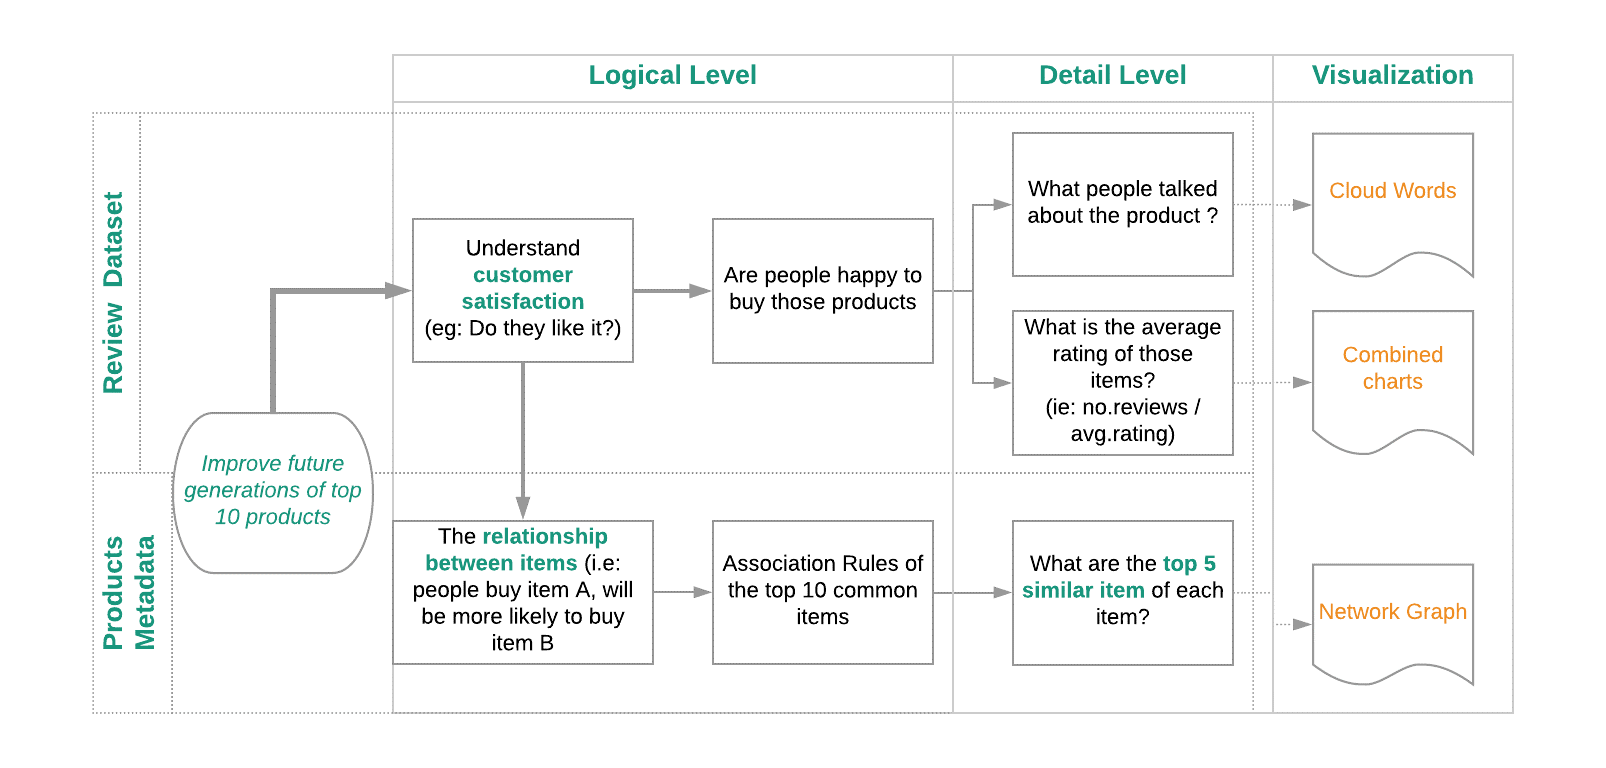
\includegraphics[width=1.1\textwidth, center]{pic1}
			\caption{Thinking Flow: Brainstorming Map}
		\end{figure}
		The horizontal containers, in the flow chart, show 2 different datasets used in the project, and the vertical ones are the question hierarchy starting with a general logical level then drilling down to specific questions, finally ending up with visualizations

		Throughout the document, we will provide images, explanation, and discoveries of the insight derived from those images

	\subsection{Problem Description}
		There are many problems we find when working on the project:
		\begin{itemize}
			\item \textbf{Dealing with big datasets} We have approximately \textbf{550,000 records each dataset}, we download data from SNAP Stanford University, but it is a raw dataset and contain a lot of redundant information
			\item \textbf{Variety of data types} such as JSON, CSV, Text, we have to do a lot of wrangling data to finally produce a formatted dataset
			\item \textbf{Slow performance queries} when we try to combine those dataset into a single table, it comes up with a huge number of records, over 7 million rows due to join tables. To solve it, we store all the data into Microsoft SQL Server database with indexing
			\item \textbf{Text processing} in the report, we try to see what customers put in the review. If they like the product, we will see some emotional words, such as “great”, “good”, “awesome”, “affordable”, “worthy”
			\item \textbf{Algorithms} in the project, we have to use Apriori algorithm to derive the insight from data. First, the frequent pattern mining, it helps us to build correlated items corresponding to a product
			\item \textbf{Network Visualization} we deal with a graph with 150 nodes and more than 700 edges for visualizing
		\end{itemize}
	
	\subsection{Limitations}
		The product metadata dataset contains over 500,000 items, but to narrow down we only analyse on \textbf{“Music Digital”} category which is over 60,000 items from 1998 to 2014. Also, the purpose of this project is to improve top 10 most popular products which is based on the number of reviews, so the document will focus on analysing only the top 10 items
		
		Even though we do a lot of wrangling data for text analysis, the cloud words seems to be less accurate than what we expect. In another word, the bag words do not represent completely the insight from reviews, some invaluable words still appear. Prefix, suffix words and collocations are not considered

	
\section{Data Wrangling}
	\subsection{Data Description}
		The datasets are downloaded from SNAP Stanford University:
		\begin{itemize}
			\item Source link: \url{http://jmcauley.ucsd.edu/data/amazon/links.html}
			\item Description: the data contains product metadata and review information 
			\item Number of digital music items: \textbf{279,899}
			\item Relevant Reviews: \textbf{836,006}
		\end{itemize}				
		
		\subsubsection{A snapshot of data}
		\textbf{Metadata Product}
		\begin{figure}[H]
			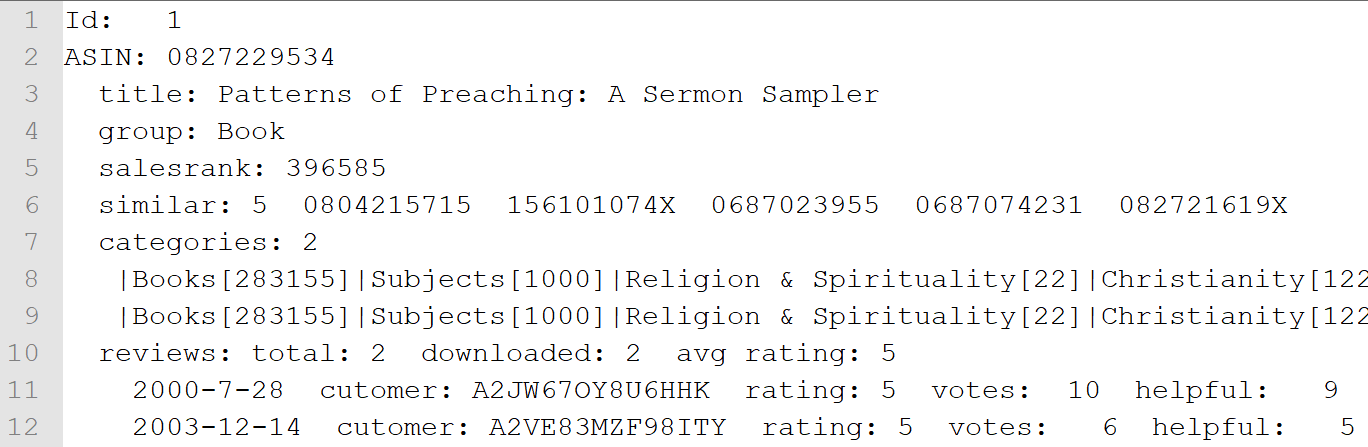
\includegraphics[width=1\textwidth, center]{pic2}
			\caption{A record uncompressing from Product Metadata}
		\end{figure}
		
		\textbf{Product Review}
		\begin{figure}[H]
			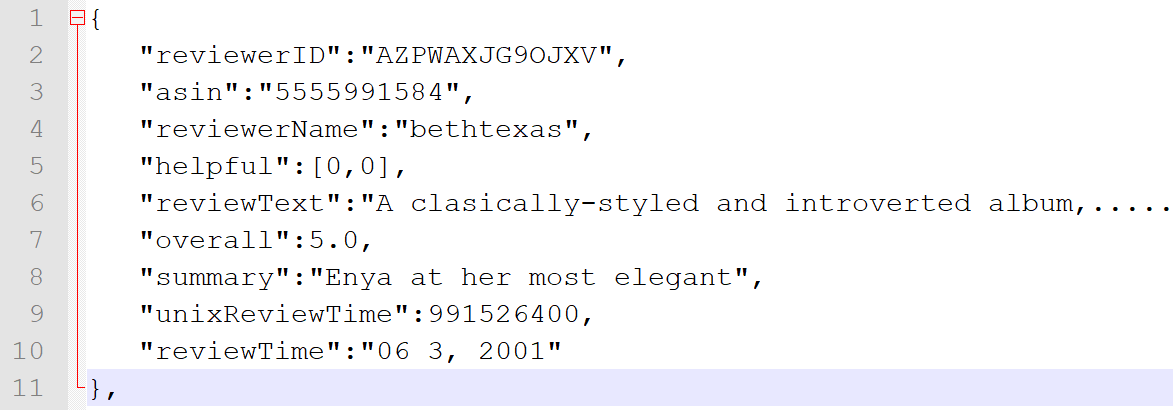
\includegraphics[width=1\textwidth, center]{pic3}
			\caption{A record uncompressing from Review json file}
		\end{figure}
		
		\subsubsection{Formatted Data Output}
		\begin{tabular}{|>{\centering\arraybackslash}p{2cm}|>{\centering\arraybackslash}p{2.5cm}|>{\centering\arraybackslash}p{2cm}||>{\arraybackslash}p{8cm}|}
		\hline 
		\textbf{Source} & \textbf{Feature} & \textbf{Type} & \textbf{Description} \\
		\hline 
		Metadata & asin & bigint & ID of the product \\ 
		\hline 
		"" & title & varchar & Title of the product / product name \\ 
		\hline 
		"" & group & varchar & Product group (Book, DVD, Music) \\ 
		\hline 
		"" & salesRank & int & Amazon sales rank \\ 
		\hline 
		"" & similar & bigint & Similar items recommended by Amazon \\ 
		\hline 
		"" & categories & varchar & Location in product category hierarchy \\ 
		\hline 
		"" & reviews & varchar & Review summary \\ 
		\hline 
		Review & reviewerId & varchar & ID of the reviewer \\ 
		\hline 
		"" & reviewerName & varchar & Name of reviewer \\ 
		\hline 
		"" & helpful & faction & Helfulness figure rated by visitors \\ 
		\hline 
		"" & reviewText & varchar & Customer review text \\ 
		\hline 
		"" & rating & decimal(2,2) & Customer rating for the product \\ 
		\hline 
		"" & reviewTime & date & Time of the review \\ 
		\hline
		\end{tabular} 
	
	\subsection{Wrangling Tools}
		\begin{tabular}{|>{\centering\arraybackslash}p{4cm}||>{\centering\arraybackslash}p{11.5cm}|}
			\hline 
			\textbf{Language} & Python 2 on Jupyter Notebook \\ 
			\hline 
			\textbf{Libraries} & Json, Pandas, Regular Express RE, NLTK, Stop words data, Corpus, wordtokenize, d3Network, ODBC \\ 
			\hline 
			\textbf{Workbooks} & Data Manipulation with Amazon Products Metadata.ipynb, Data Manipulation with Amazon Reviews Data.ipynb \\ 
			\hline 
			\end{tabular} 	
	
	\subsection{Text Data Processing}
		\begin{figure}[H]
			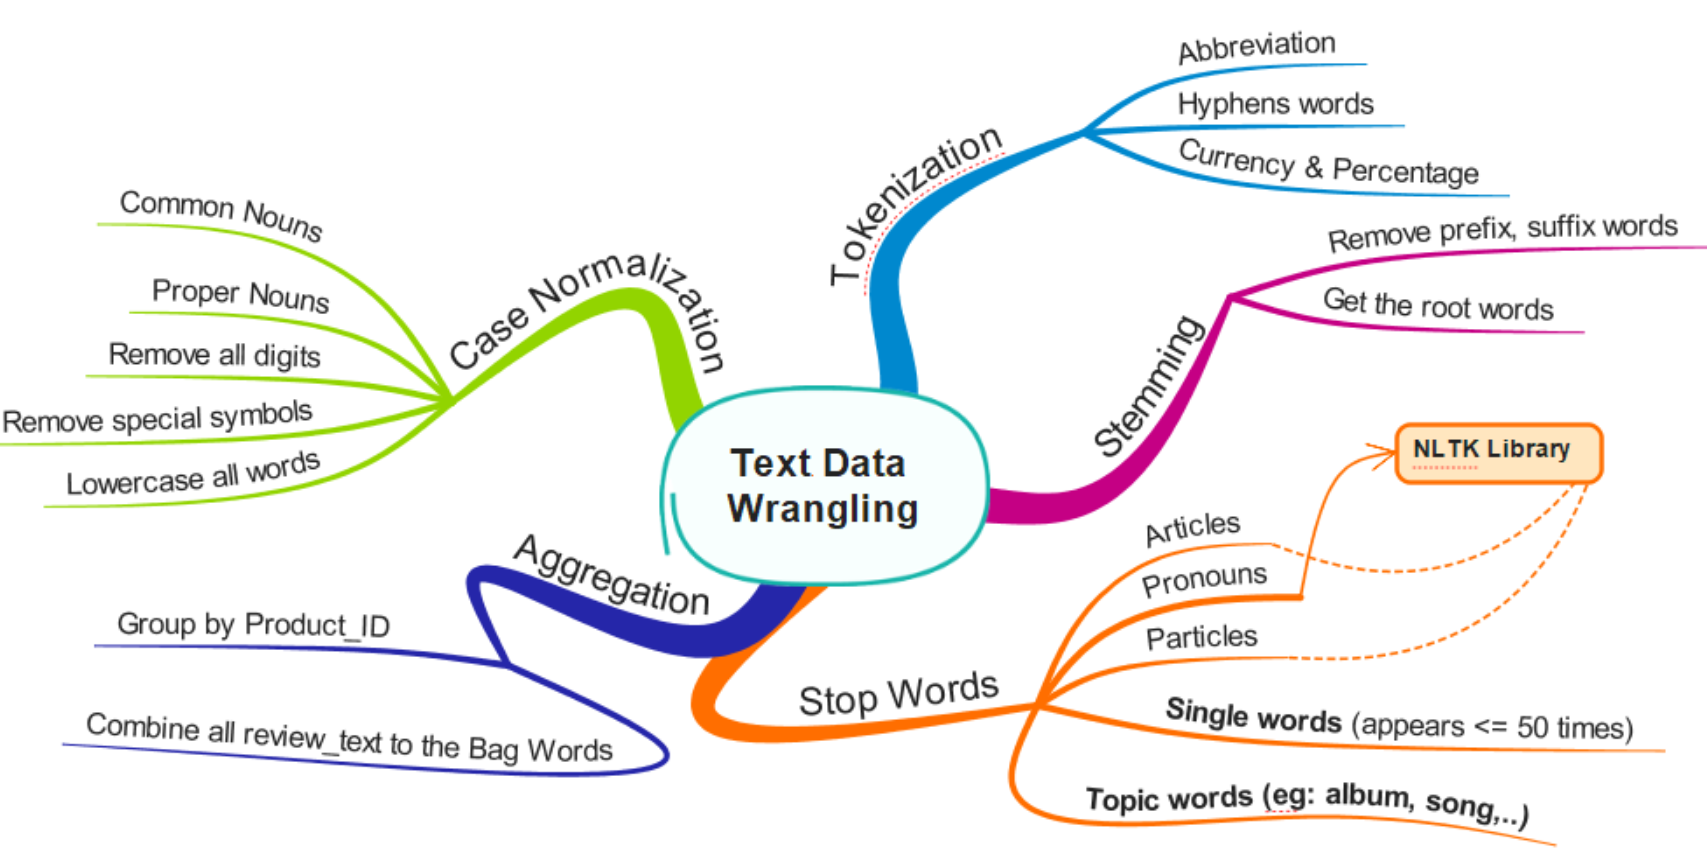
\includegraphics[width=1.2\textwidth, center]{pic4}
			\caption{Mindmap: Steps for Text data wrangling}
		\end{figure}
		
		\textbf{What we have done to wrangle the raw text data:}
		\begin{enumerate}
			\item \textbf{Loading data}
				\begin{itemize}
					\item Parsing json file
					\item Normalizing data, save it in Pandas
				\end{itemize}
			\item \textbf{Formatting data}
				\begin{itemize}
					\item Checking data format
					\item Standardize "helpful" from faction into right format
				\end{itemize}
			\item \textbf{Tokenization}
				\begin{itemize}
					\item Hyphen words removed
					\item Currency %&% percentage %&% special symbols removed
				\end{itemize}
			\item \textbf{Stop Words}
				\begin{itemize}
					\item Stop words list from NLTK library
					\item Single word (words appear one in the text)
					\item Remove topic words, such as "album", "song", "instrument", "music"
				\end{itemize}
			\item \textbf{Aggregating}
				\begin{itemize}
					\item Group data by product%_%id
					\item Combine all "review%_%text" to a Bag word
				\end{itemize}
			\item \textbf{Performance enhancement}
				\begin{itemize}
					\item Store all data into tables in MS SQL Server, because data is too big to export
				\end{itemize}
		\end{enumerate}				
		
		\textbf{Finally, we have a clean dataset stored in Microsoft SQL tables}
		\begin{figure}[H]
			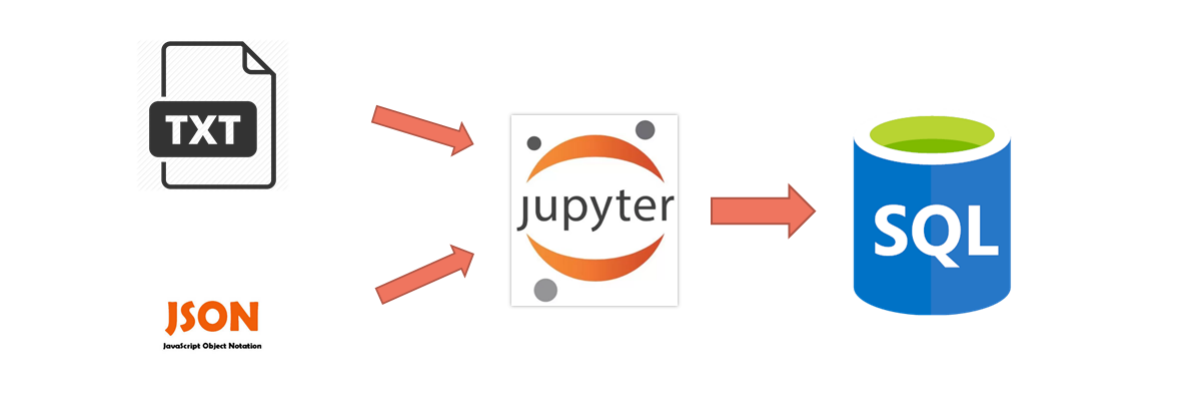
\includegraphics[width=1\textwidth, center]{pic5}
			\caption{Mindmap: Steps for Text data wrangling}
		\end{figure}
		
	\subsection{Text Analysis}
	\textbf{Problem 1:} after combining all review texts of the first item. We see a lot of less informative words, such as "quote", "album", "song", "one", "music"
	\begin{figure}[H]
		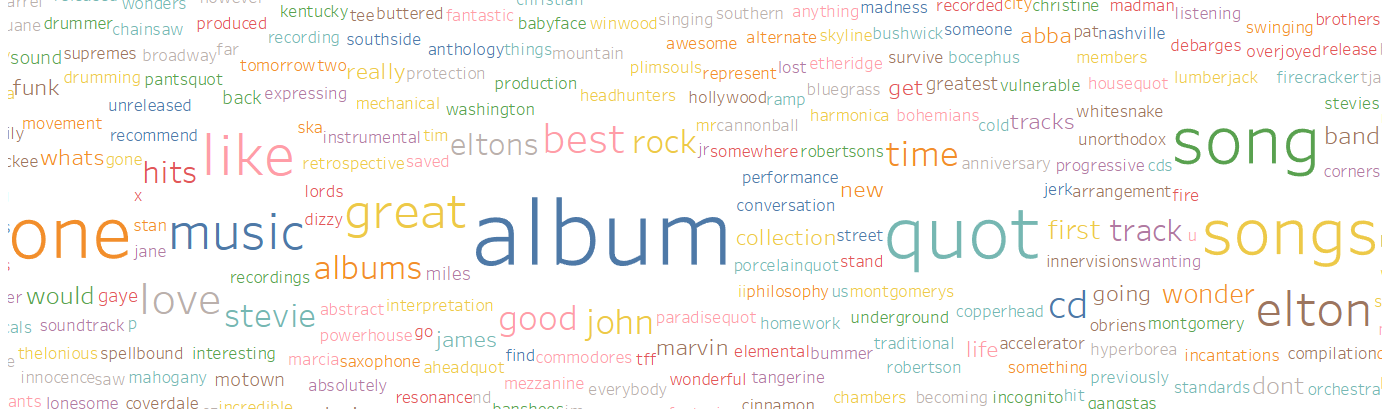
\includegraphics[width=1\textwidth, center]{pic6}
		\caption{Cloud word before removing topic words}
	\end{figure}	
	\textbf{Solution 1: We collect topic words, and insert them into stop words list. Single words are also considered}
	
	\textbf{Problem 2:} Aggregating data for network graph visualization is not easy. We have to convert relational data into nodes, and edges format, so that the \textit{“d3Network”} library can process. 
	
	Also, we have a lot of edges and nodes at the end, this is not practical to visualize
	\textbf{Solution 2:} Removing all nodes have less than 5 connections, and use D3js to visualize data
	
\section{Data Checking}
	\subsection{Data Distribution with Histogram}
		\begin{figure}[H]
			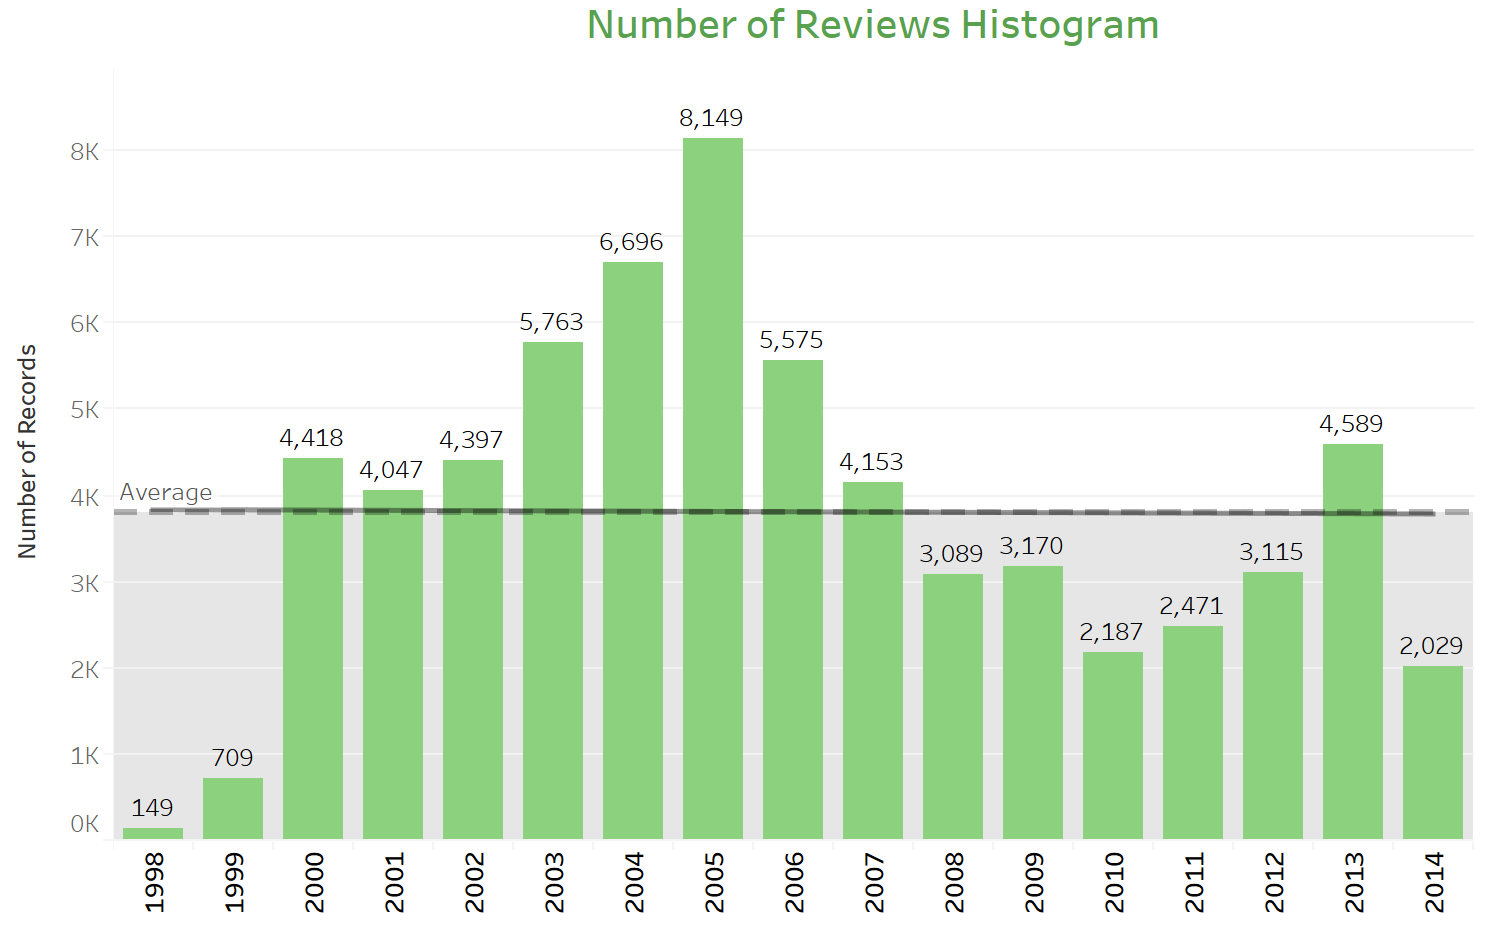
\includegraphics[width=1\textwidth, center]{pic7}
			\caption{Histogram: number of reviews from 1998 to 2014}
		\end{figure}	
		The graph illustrates the distribution of reviews over years from 1998 to 2014. The dash line stands for the average review number which is nearly 4000 over 17 years period
		
		We can see that the maximum number in 2005 which is 8.149 reviews, but in 2010 the figure went down significantly to 2,187 due to the financial crisis since 2008
		
		At the beginning in 1988, Amazon didn’t have many products, therefore the number was very low

	
\section{Data Exploration}
	\subsection{What are the top 10 highest reviews?}
	The diagram shows top 10 items that have highest number of reviews from 1998 to 2014. In the container, there are 3 labels that are ASIN, Title of product, number of reviews respectively
	\begin{figure}[H]
			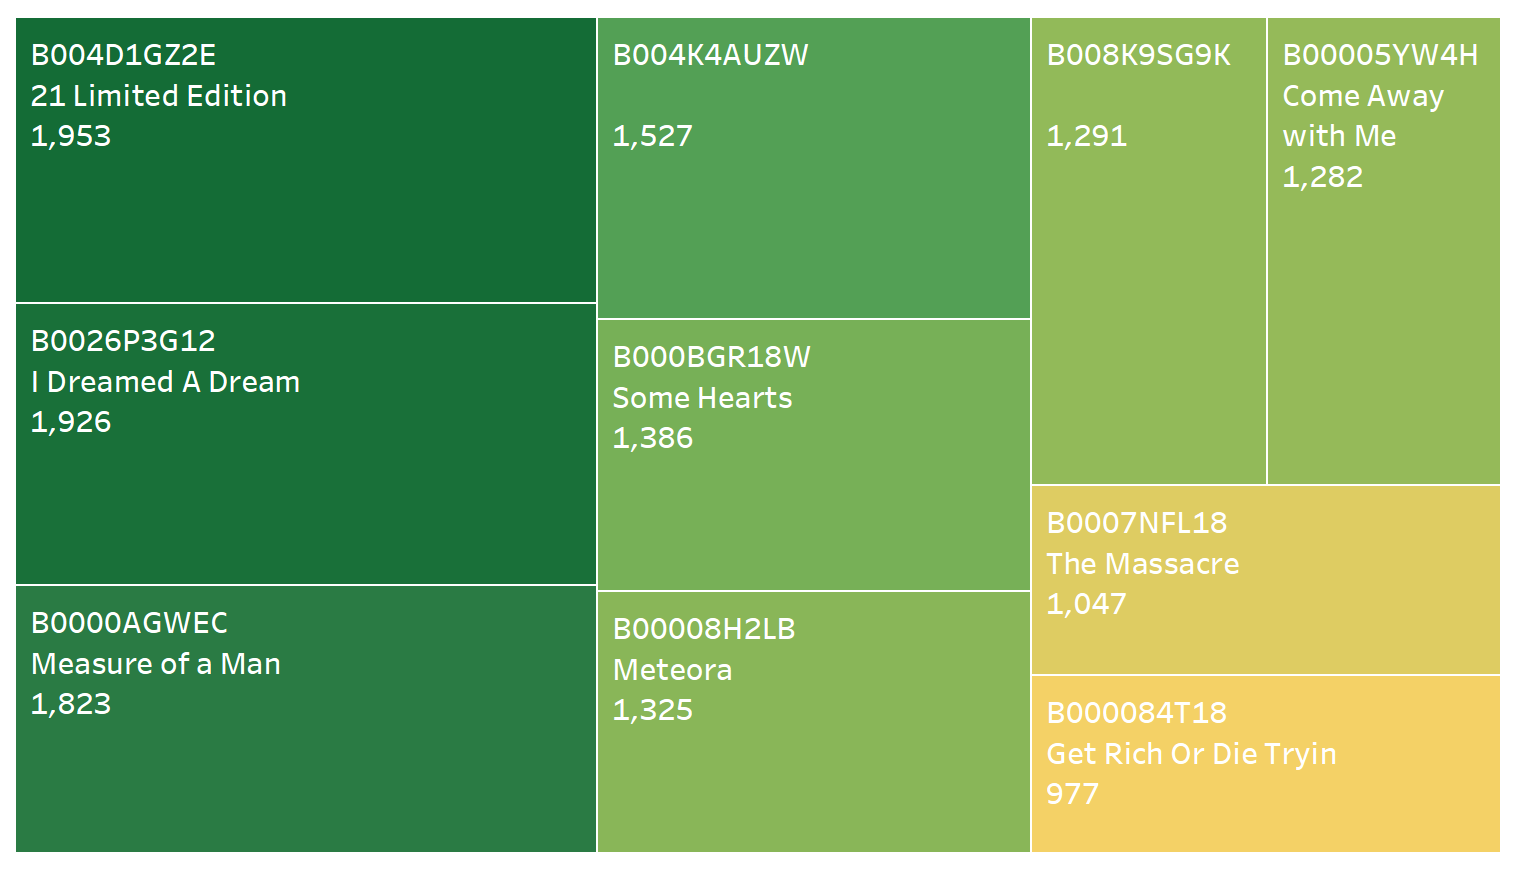
\includegraphics[width=1\textwidth, center]{pic8}
			\caption{Top 10 albums have highest reviews from 1989 to 2014}
	\end{figure}	
	
	
	\subsection{Are people happy to buy those items?}
		The exploration process for this question includes 2 main steps:
		\begin{itemize}
			\item Firstly, building a bag of words, we can see what keywords they use to describe the product, whether they are positive or negative words
			\item Secondly, we look at the average rating by customers against the number of reviews. This shows what rate customers give for each product
		\end{itemize}
	
		\subsubsection{What did they talk about those products?}
			To concentrate on analysing at detail, we will look at the top 1 album which is \textit{“B004D1GZ2E”,Adele: 21 Limited Edition album,} in the ASIN Amazon product identification
			
			
			\textbf{Data Preparation Process}
			\begin{itemize}
				\item We clean the whole “review” dataset by removing symbols, digits
				\item Merging all review texts to a single paragraph
				\item Tokenizing the paragraph, meaning that we split it by word and store them in a long list
				\item Creating a “stop words” list which is defined by
				\begin{itemize}
					\item Articles, pronouns, particles which are supported by NLTK library in Python
					\item Single word which is the word appears only one in the paragraph
					\item Look at top 100 most frequent words only
				\end{itemize}
				\item Saving the bag words result in MS SQL tables
				\item Using Tableau to visualize data
			\end{itemize}
			
			
			\textbf{Statistical Summary table}
			
			\begin{tabular}{|>{\arraybackslash}p{9cm}||>{\centering\arraybackslash}p{5cm}|}
						\hline 
						\textbf{Feature} & \textbf{Value} \\ 
						\hline 
						Total number of Reviews & 1,953 \\ 
						\hline 
						Total number of words in praragraph & 112,868 \\ 
						\hline 
						Total number of stop words removed & 62,291 \\ 
						\hline 
						Total number in Bag words & 13,924 \\ 
						\hline 
			\end{tabular}
			
			
			\textbf{Visualization}		
			\begin{figure}[H]
				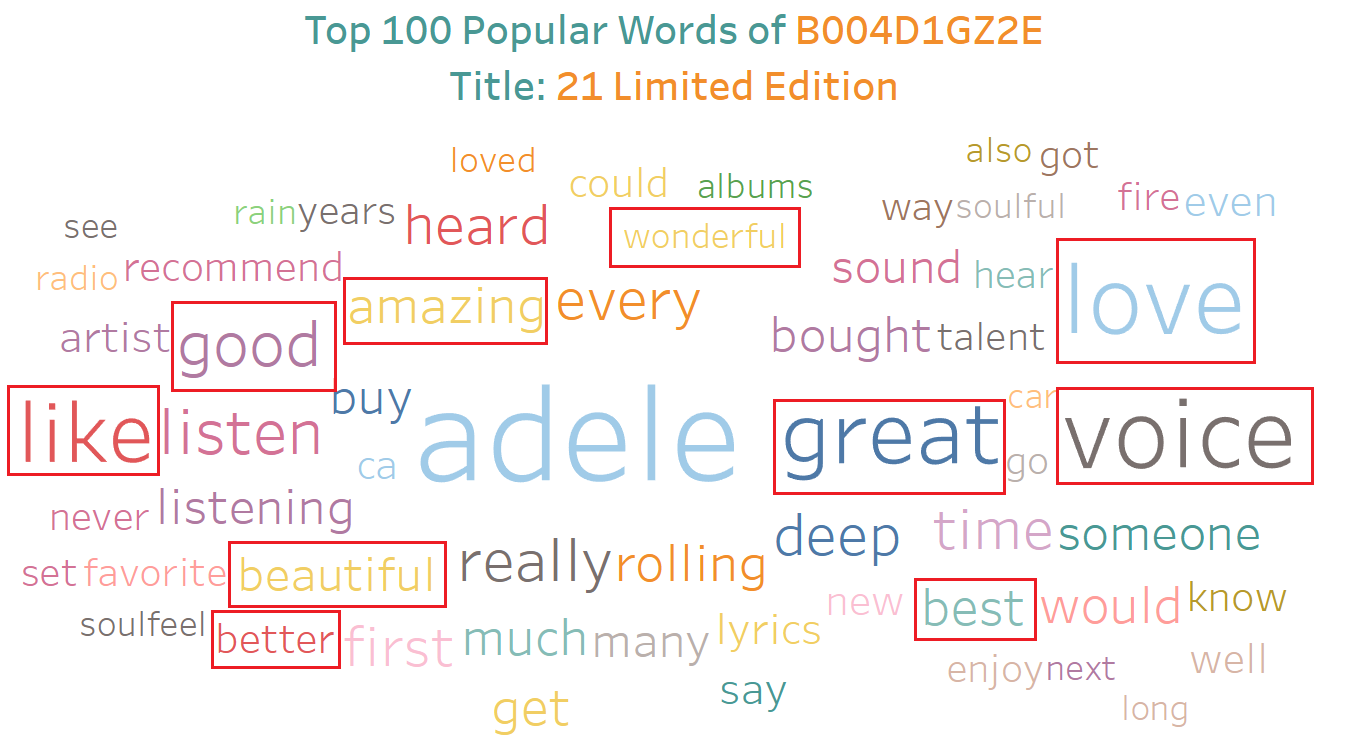
\includegraphics[width=1\textwidth, center]{pic9}
				\caption{Cloud Words of album "Adele: 21 Limited Edition" with Tableau}
			\end{figure}	
			
			
			\textbf{Discoveries}
			\begin{itemize}
				\item Looking at the graph, we can see that people say “good”, “amazing”, “wonderful”, and “adele”
				\item Indeed, “21 Limited Edition” is the best album of Adele since 2011. It achieved a lot of awards, such as Grammy Awards for album of the year
				\item By looking at the visualization, we can see that audiences like her album, and one of the reasons is because of her voice
			\end{itemize}
		
			
			\textbf{Limitations}
			\begin{itemize}
				\item The result is not as good as what we expect. This is because we couldn’t get rid of prefix, suffix of a word to get the root. For example, “song” and “songs” are the same meaning, so they should be combined into one word
				\item Collocation should be considered. At the moment, we just consider only single word
			\end{itemize}						
			
		\subsubsection{What is the average rating against reviews?}
		We want to see the correlation between “average rating” and “number of reviews” for top 10 most popular items in 2014. Whether or not the albums with highest reviews were also high ranking
		
		
		\textbf{Visualization}
		\begin{figure}[H]
				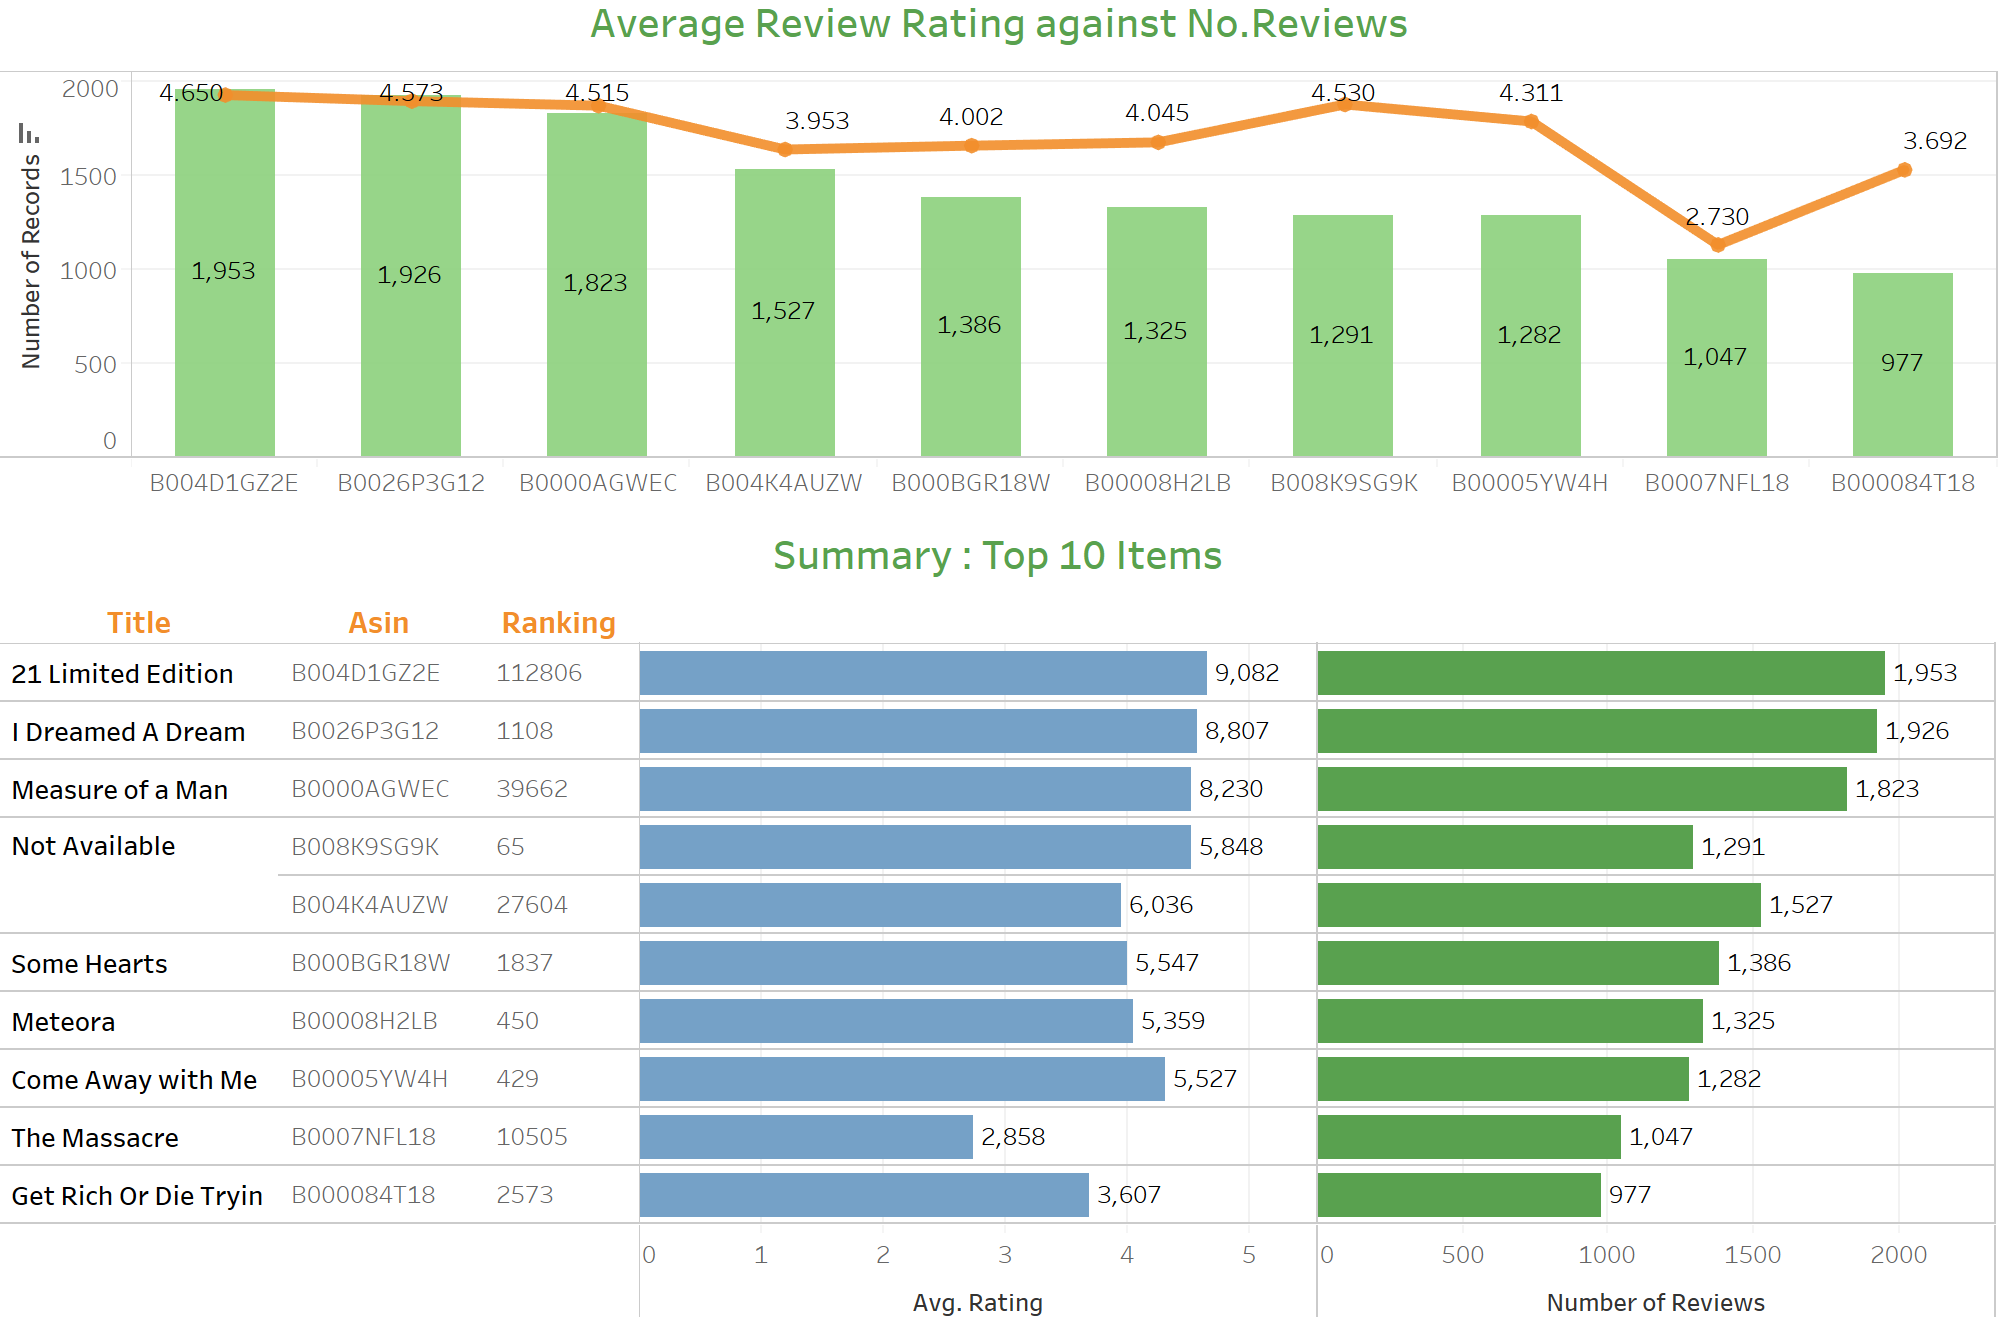
\includegraphics[width=1\textwidth, center]{pic10}
				\caption{Dashboard: Average review rating against No.Reviews}
		\end{figure}	
		
		
		\textbf{Discoveries}
		\begin{itemize}
			\item The graph demonstrates top 3 items have the highest rating, meaning that they are very good product with high sales, high review and high ranking
			\item However, the “Come Away with Me” album had a very high ranking and rating, but the reviews were low. It is also a worthy product to buy
			\item “The Massacre” had 1,047 reviews in 2014, but the rating was just 2.73. it seems to me that it’s not a really good album to keep
		\end{itemize}
		
		
		\textbf{Limitations}
		\begin{itemize}
			\item The number of features available is short, so that we can’t build a correlation matrix to see a bigger picture of data
		\end{itemize}
	
	\subsection{What the relationship looks like between items?}
		There is a real demand that customers have demands, but they don’t know what they should buy actually. By using recommendation system, we can recommend them which products are similar to what they are looking for
		
		In the section, we introduce the results of \textbf{“Apriori”} algorithm by visualizing it on an interactive Network Graph in R with D3js

		
		\textbf{Exploration Process}
		\begin{itemize}
			\item We have over 80 thousand items in the database, this is not practical to put all of them into the network graph. Thus, we select only top 15 items of highest reviews
			\item From the metadata product, we can extract the frequency of each item (ie: asin code). All items with frequency less than 5 will be removed. In another word, we just keep nodes with more than 5 edges. At the end, we will have a list of itemset
			\item Store it into 2 tables in MS SQL Server for visualization
			\item In R, we used \textbf{“d3Network”} which generates interactive network visualizations using D3 javascript library
		\end{itemize}
		

		\textbf{Visualization and Discoveries}
		\begin{figure}[H]
				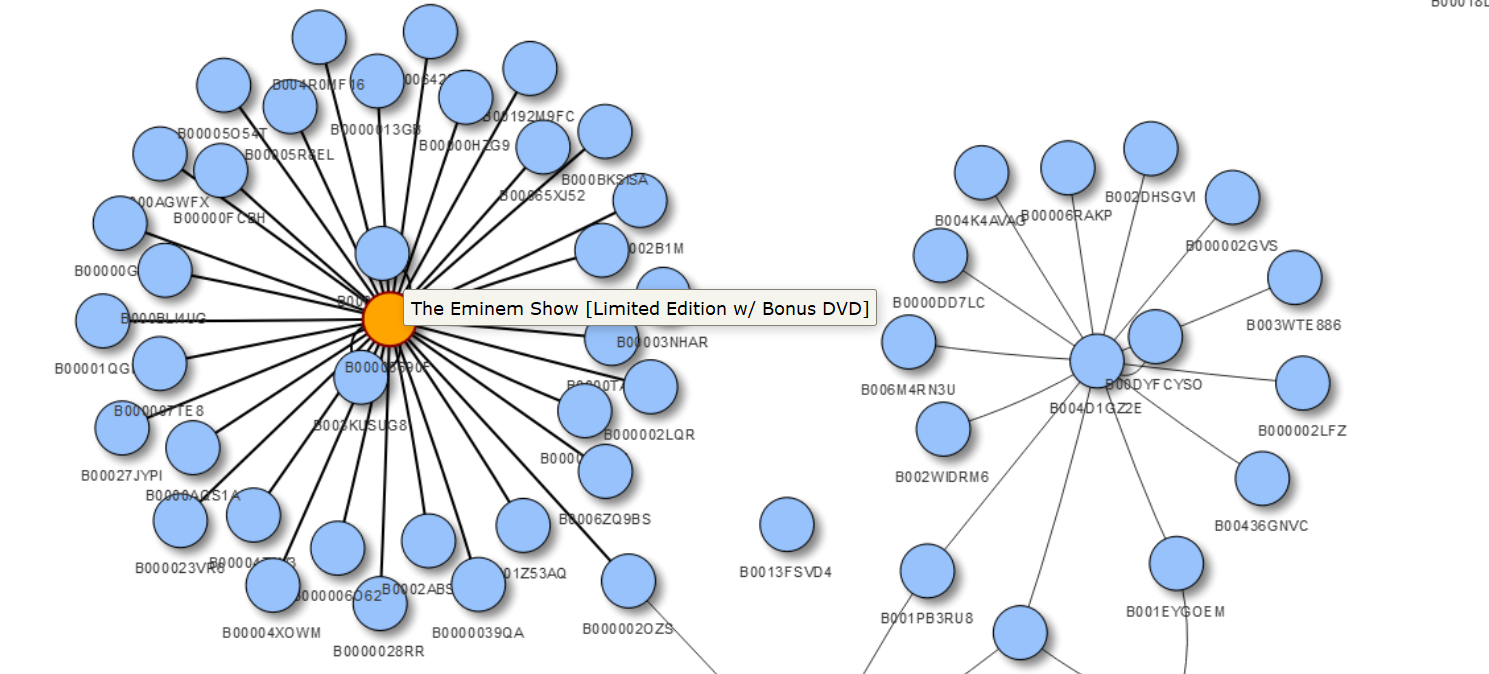
\includegraphics[width=1\textwidth, center]{pic11}
				\caption{The network graph, the centroid is node which is linked to other similar node in the network}
		\end{figure}	
		“The Eminem Show” has most connections from other nodes. This means it is the most popular item in Amazon in 2014
		\begin{figure}[H]
				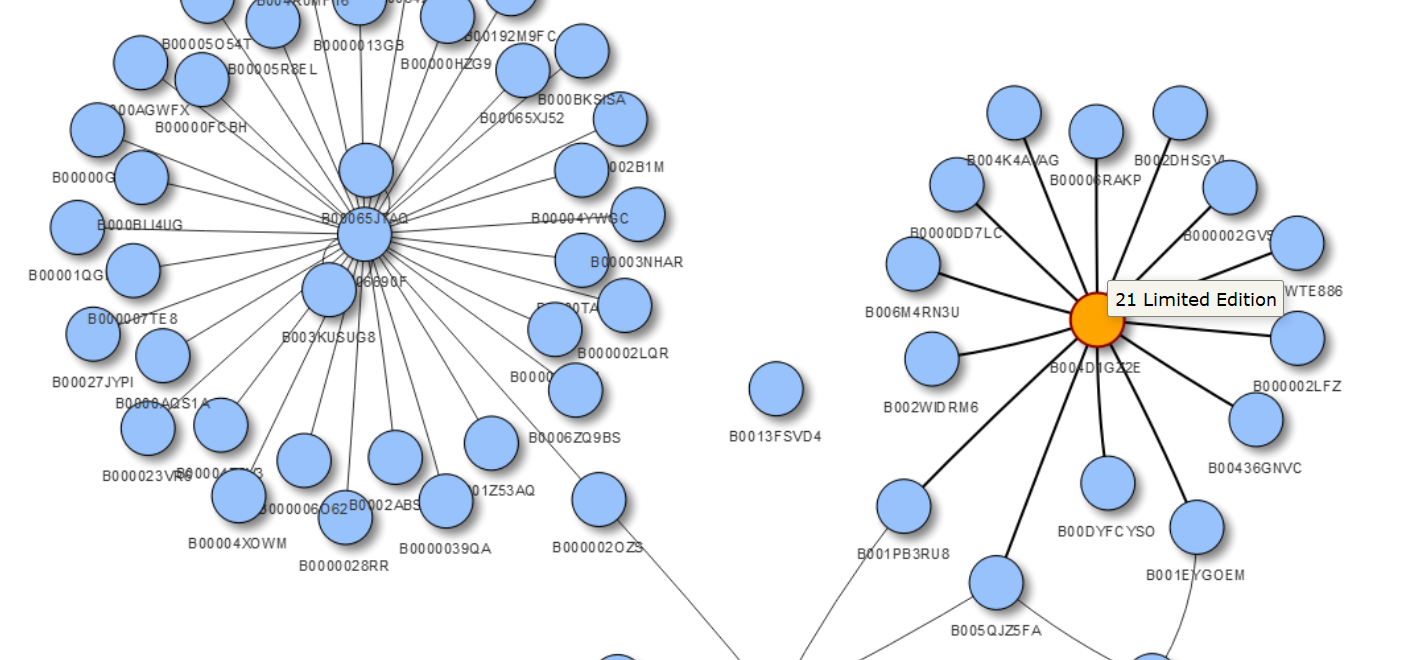
\includegraphics[width=1\textwidth, center]{pic12}
		\end{figure}	
		The second one is “21 Limited Edition” of Adele. Although it has less connection than “The Eminem Show”, it has the most reviews in 2014

		By looking at the big image, we can see what albums customers pay attention in 2014. Also, those items had high demand in the past

\section{Conclusion}
	I have worked in different stages in the process of analysing data from the scratch. I have to read different materials to choose a right data source which fits the project's tasks, and my capability
	
	At the beginning, it was difficult to deal with a big dataset. Also, the data is not in the right format, which requires me to wrangling a lots
	
	After the ideas to analyse data, it's challenging as well, because most of the ideas is not suitable with the dataset. However, if i merge many different datasets, it will be not enough time to finish the project
	
	Visualization tools is very interesting, especially when i work with D3js and Shiny. I have learnt a lot of new things from the project by going through different stages of analysing data. Now it is the time to create a web-based with interactive visualizations to communicate the results

\section{References}
	\begin{itemize}
		\item D3Network. (n.d.). Retrieved from \url{http://christophergandrud.github.io/d3Network/}
		\item Apriori algorithm. (2018, February 17). Retrieved from \url{https://en.wikipedia.org/wiki/Apriori_algorithm}
		\item Static and dynamic network visualization with R. (n.d.). Retrieved from \url{http://kateto.net/network-visualization}
		\item R. He, J. McAuley. Modeling the visual evolution of fashion trends with one-class collaborative filtering. WWW, 2016
		\item J. McAuley, C. Targett, J. Shi, A. van den Hengel. Image-based recommendations on styles and substitutes. SIGIR, 2015

	\end{itemize}







\end{document}